The Displacement-based Earthquake Loss Assessment (DBELA) methodology permits the calculation of the displacement capacity of a collection of structures at a number of limit states (which could be structural or non-structural). These displacements are derived based on the capacity of an equivalent SDoF structure, following the principles of structural mechanics (\cite{CrowleyEtAl2004}; \cite{BalEtAl2010}; \cite{SilvaEtAl2013}).\\
The displacement at the height of the centre of seismic force of the original structure ($H_{CSF}$) can be estimated by multiplying the base rotation by the height of the equivalent SDoF structure ($H_{SDOF}$), which is obtained by multiplying the total height of the actual structure ($H_T$) by an effective height ratio ($ef_h$), as illustrated in Figure~\ref{fig:efh}:

\begin{figure}[htb]
  \centering
      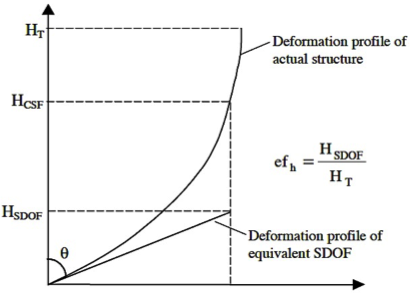
\includegraphics[width=8cm]{figures/effective_height.png}
  \caption{Definition of effective height coefficient \cite{GlaisterPinho2003}.}
  \label{fig:efh}
\end{figure}

\cite{PinhoEtAl2002} and \cite{GlaisterPinho2003} proposed formulae for estimating the effective height coefficient for different response mechanisms. For what concerns the beam sway mechanism (or distributed plasticity mechanism, as shown in Figure \ref{fig:mechanisms}), a ratio of 0.64 is proposed for structures with 4 or less storeys, and 0.44 for structures with 20 or more storeys. For any structures that might fall within these limits, linear interpolation should be employed. With regards to the column-sway mechanism (or concentrated plasticity mechanism, as shown in Figure~\ref{fig:mechanisms}), the deformed shapes vary from a linear profile (pre-yield) to a non-linear profile (post-yield). As described in \cite{GlaisterPinho2003}, a coefficient of 0.67 is assumed for the pre-yield response and the following simplified formula can be applied post-yield (to attempt to account for the ductility dependence of the effective height post-yield coefficient):

\begin{equation}
  ef_h = 0.67 - 0.17\frac{\epsilon_{s(LS_i)}-\epsilon_y}{\epsilon_{s(LS_i)}}
\end{equation}

\begin{figure}[htb]
  \centering
      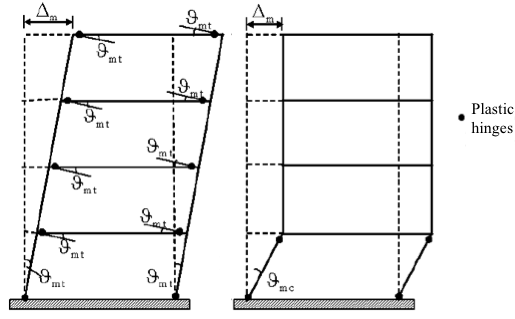
\includegraphics[width=10cm]{figures/collapse_mechanisms.png}
  \caption{Deformed profiles for beam-sway (left) and column-sway (right) mechanisms\cite{PaulayPriestley2002}.}
  \label{fig:mechanisms}
\end{figure}
The displacement capacity at different limit states (either at yield ($\delta_y$) or post-yield ($\delta_{(LSi)}$) for bare frame or infilled reinforced concrete structures can be computed using simplified formulae, which are distinct if the structure is expected to exhibit a beam- or column-sway failure mechanism. These formulae can be found in \cite{BalEtAl2010} or \cite{SilvaEtAl2013}, and their mathematical formulation is described in detail in \cite{CrowleyEtAl2004}.\\

In order to estimate whether a given frame will respond with a beam- or a column-sway mechanism it is necessary to evaluate the properties of the storey. A deformation-based index ($R$) has been proposed by \cite{AboElEzz2008} which reflects the relation between the stiffness of the beams and columns. This index can be computed using the following formula:
\begin{equation}
R = \frac{^{h_b}/_{l_b}}{^{h_c}/_{l_c}}
\end{equation}

Where $l_c$ stands for the column length. \cite{AboElEzz2008} proposed some limits for this index applicable to bare and fully infilled frame structures, as described in Table \ref{table:AboElEzz2008}.
\begin {table}[htb]
\caption{Limits for the deformation-based sway index proposed by \cite{AboElEzz2008}}
\label{table:AboElEzz2008}
\begin{center}
  \begin{tabular}{ | c | c | c |}
  \hline
    Building Typology & Beam sway & Column sway  \\ \hline
    Bare frames & R$\leq$1.0 & R>1.5 \\ \hline
    Fully infilled frames & R$\leq$1.0 & R>1.0 \\ \hline
  \end{tabular}
\end{center}
\end{table}

The calculation of the corresponding spectral acceleration is performed by assuming a perfectly elasto-plastic behaviour. Thus, the spectral displacement for the yielding point is used to derive the associated acceleration through the following formula:

\begin{equation}
Sa_i = \frac{4\pi^2Sd_i}{T_y^2}
\end{equation}

Where $T_y$ stands for the yielding period which can be calculated using simplified formulae (e.g. \cite{CrowleyPinho2004}; \cite{CrowleyPinho2006}), as further explained in Section~\ref{subsec:DBELA_Silva2013}. Due to the assumption of the elasto-plastic behaviour, the spectral acceleration for the remaining limit states (or spectral displacements) will be the same (see Figure~\ref{fig:DBELA_cc}).\\

In order to use this methodology it is necessary to define a building model, which specifies the probabilistic distribution of the geometrical and material properties. This information is currently stored in a $csv$ file (tabular format), as presented in Table~\ref{table:building_model_dbela}.

\begin {table}[htb]
\caption{Example of a building model compatible with the DBELA method.}
\label{table:building_model_dbela}
\begin{center}
  \begin{tabular}{ | l | l | l | l | l | l |}
  \hline
Structure type & bare frame &  &  &  &  \\ \hline
ductility & ductile &  &  &  &  \\ \hline
number of storeys & 3 &  &  &  &  \\ \hline
steel modulus & lognormal & 210000 & 0.01 & 0 & inf \\ \hline
steel yield strength & normal & 371.33 & 0.24 & 0 & inf \\ \hline
ground floor height & discrete & 2.8 3.1 3.2 & 0.48 0.15 0.37 & 0 & inf \\ \hline
regular floor height & lognormal & 2.84 & 0.08 & 0 & inf \\ \hline
column depth & lognormal & 0.45 & 0.12 & 0.3 & 0.6 \\ \hline
beam length & gamma & 3.37 & 0.38 & 0 & inf \\ \hline
beam depth & lognormal & 0.6 & 0.16 & 0.4 & 0.8 \\ \hline
  \end{tabular}
\end{center}
\end{table}

The \verb=structure type= can be set to \verb=bare frame= or \verb=infilled frame=, while the parameter \verb=ductility= can be equal to \verb=ductile= or \verb=non-ductile=. The variable \verb=number of storeys= must be equal to an integer defining the number of floors of the building class. The following parameters (\verb=steel modulus= , \verb=steel yield strength= , \verb=ground floor height= , \verb=regular floor height= , \verb=column depth= , \verb=beam length= , \verb=beam depth=) represent the geometrical and material properties of the building class, and can defined in a probabilistic manner. Currently, three parametric statistical models have been implemented (\verb=normal= , \verb=lognormal= and \verb=gamma=), as well as the discrete (i.e. probability mass function) model (\verb=discrete=). The model that should be used must be specified on the second column. Then, for the former type of models (parametric), the mean and coefficient of variation should be provided in the third and fourth columns, respectively. For the discrete model, the central values of the bins and corresponding probabilities of occurrence should be defined in the third and fourth columns, respectively. The last two columns can be used to truncate the probabilistic distribution between a minimum (fifth column) and maximum (sixth column) values. In order to define a parameter in a deterministic manner (i.e. no variability), the coefficient of variation for the associated attribute can be set to zero, and the same value (mean) will be used repeatedly.\\

The location of the building model and the damage model (see Section \ref{subsec:dmg_model}) should be specified in the variables \verb=building_model= and the \verb=damage_model=, respectively. The number of capacity curves that should be generated must be defined using the parameter \verb=no_assets=. Then, after importing the module \verb=DBELA=, the set of capacity curves can be generated using the following commands:

\begin{Verbatim}[frame=single, commandchars=\\\{\}, samepage=true]
building_class_model = DBELA.read_building_class_model(building_model)
assets = DBELA.generate_assets(building_class_model,no_assets)
capacity_curves = DBELA.generate_capacity_curves(assets,damage_model)
\end{Verbatim}

The first function (\verb=read_building_class_model=) processes the information about the building class; the second function (\verb=generate_assets=) uses a Monte Carlo sampling process to generate a set of synthetic structural models (each one with unique geometrical and material properties); and the final function (\verb=generate_capacity_curves=) combines the generated assets with the damage model to calculate a capacity curve per structure. Figure \ref{fig:DBELA_cc} presents a collection of capacity curves generated using this methodology.

\begin{figure}[htb]
  \centering
      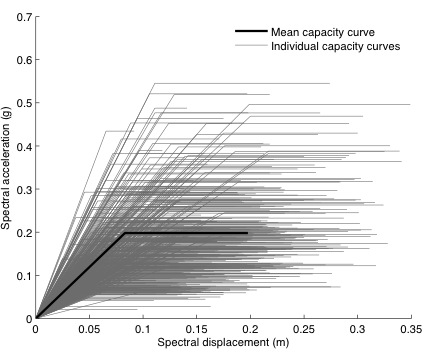
\includegraphics[width=8cm]{figures/synthethic_capacity_curves.png}
  \caption{Capacity curves for reinforced concrete bare frames generated using the DBELA methodology.}
  \label{fig:DBELA_cc}
\end{figure}